% This LaTeX was auto-generated from MATLAB code.
% To make changes, update the MATLAB code and export to LaTeX again.

\documentclass{article}

\usepackage[utf8]{inputenc}
\usepackage[T1]{fontenc}
\usepackage{lmodern}
\usepackage{graphicx}
\usepackage{color}
\usepackage{hyperref}
\usepackage{amsmath}
\usepackage{amsfonts}
\usepackage{epstopdf}
\usepackage[table]{xcolor}
\usepackage{matlab}

\sloppy
\epstopdfsetup{outdir=./}
\graphicspath{ {./assignment_1_images/} }

\begin{document}

\matlabtitle{Robot Mobility: Assignment 1}

\begin{par}
\begin{flushleft}
Submitted by: Sushanth Jayanth
\end{flushleft}
\end{par}


\matlabheading{\includegraphics[width=\maxwidth{56.39739086803814em}]{image_0}}

\begin{par}
\begin{flushleft}
\includegraphics[width=\maxwidth{56.49774209734069em}]{image_1}
\end{flushleft}
\end{par}

\begin{par}
\begin{flushleft}
\includegraphics[width=\maxwidth{56.49774209734069em}]{image_2}
\end{flushleft}
\end{par}

\begin{par}
\begin{flushleft}
\includegraphics[width=\maxwidth{56.69844455594581em}]{image_3}
\end{flushleft}
\end{par}

\begin{par}
\begin{flushleft}
\includegraphics[width=\maxwidth{56.297039638735576em}]{image_4}
\end{flushleft}
\end{par}

\begin{par}
\begin{flushleft}
\includegraphics[width=\maxwidth{56.69844455594581em}]{image_5}
\end{flushleft}
\end{par}



\vspace{1em}

\vspace{1em}
\matlabheading{Q 2. }

\matlabheadingthree{2 The system to be modelled has the following matrices}


\vspace{1em}
\begin{matlabcode}
% syms C_af C_ar l_f l_r I_z V_x m
I_z = 2873;
V_x = 30;
m = 1573;
C_af = 80000;
C_ar = 80000;
l_r = 1.58;
l_f = 1.1;

A = [[0,1,0,0];[0, (2*(-C_af-C_ar))/(m*V_x), (2*(C_af+C_ar))/m, (-2*(C_af*l_f - C_ar*l_r))/(m*V_x)];
    [0,0,0,1];[0, (-2*(C_af*l_f - C_ar*l_r))/(I_z*V_x), (2*(C_af*l_f - C_ar*l_r))/I_z, (-2*(C_af*l_f*l_f + C_ar*l_r*l_r))/(I_z*V_x)]]
\end{matlabcode}
\begin{matlaboutput}
A = 4x4    
         0    1.0000         0         0
         0   -6.7811  203.4329    1.6275
         0         0         0    1.0000
         0    0.8911  -26.7316   -6.8804

\end{matlaboutput}
\begin{matlabcode}

B_1 = [0; ((2*C_af)/m); 0; (2*C_af*l_f)/I_z]
\end{matlabcode}
\begin{matlaboutput}
B_1 = 4x1    
         0
  101.7165
         0
   61.2600

\end{matlaboutput}
\begin{matlabcode}

B_2 = [0; (-2*(C_af*l_f - C_ar*l_r))/(m*V_x) - V_x; 0; (-2*(C_af*l_f*l_f + C_ar*l_r*l_r))/(I_z*V_x)]
\end{matlabcode}
\begin{matlaboutput}
B_2 = 4x1    
         0
  -28.3725
         0
   -6.8804

\end{matlaboutput}


\vspace{1em}
\matlabheadingthree{ \textbf{2 d. Finding the optimal feedback control gain }}

\begin{par}
\hfill \break
\end{par}

\begin{matlabcode}
Q = [[3000,0,0,0];[0,105,0,0];[0,0,1000,0];[0,0,0,3200]];
R = 115;

K = lqr(A, B_1, Q, R)
\end{matlabcode}
\begin{matlaboutput}
K = 1x4    
    5.1075    0.7743   29.6559    4.2458

\end{matlaboutput}

\begin{par}
\begin{flushleft}
Define the trajectory parameters
\end{flushleft}
\end{par}

\begin{par}
\begin{flushleft}
The desired trajectory was divided into three zones as seen below:
\end{flushleft}
\end{par}

\begin{par}
\begin{flushleft}
\includegraphics[width=\maxwidth{56.79879578524837em}]{image_6}
\end{flushleft}
\end{par}

\begin{par}
\begin{flushleft}
The time taken to complete each zone is calculated below:
\end{flushleft}
\end{par}

\begin{matlabcode}
t_1 = 5/V_x;
t_2 = 90/V_x;
% zone 3 was extended to observe convergence times
% zone 3 which is originally 5 metres, was extended to 30 metres
t_3 = 30/V_x;

% Combined timespans
timespan = 0 : 0.03 : (t_1 + t_2 + t_3);
\end{matlabcode}


\vspace{1em}
\begin{matlabcode}
% Creating the Desired Trajectory

x_des = [];
y_des = [];

for t = timespan
    % save the x_position at every timestep
    x_des(end+1) = V_x*t;

    % save the y_position at every timestep
    if (round(t_1,2) < t) && (t < round((t_1+t_2),2))
        y_des(end+1) = 0.0556*(x_des(end)-5) - 5;
    
    elseif (t > round((t_1+t_2),2)) || (t > round((t_1+t_2),2) - 0.001)
        y_des(end+1) = 0;
    else
        y_des(end+1) = -5;
    end
end

% plot(x_des, y_des)
\end{matlabcode}


\vspace{1em}
\begin{par}
\begin{flushleft}
Create the inputs psi\_des
\end{flushleft}
\end{par}

\begin{matlabcode}
global left_turn;
global right_turn;
left_turn = 0;
right_turn = 0;

psi_dot_desired = [];
psi_desired = [];

for t=timespan
    if t < round(t_1,2)
        psi_desired(end+1) = 0;
    elseif t < round(t_2,2)
        psi_desired(end+1) = atan(1/18);
    else
        psi_desired = 0;
    end
end

% build the psi_dot_desi input

% build the psi_dot_desired input
for t = timespan
    if (round(t_1,2)-0.04 < t) && (t < 0.04+round((t_1),2)) && left_turn < 1
        % turn left
        psi_dot_desired(end+1) = atan(1/18)/0.03;
        left_turn = left_turn + 1;
    elseif (round(t_2,2)-0.04 < t) && (t < 0.04+round((t_2),2)) && right_turn < 1
        % turn right
        psi_dot_desired(end+1) = -atan(1/18)/0.03;
        right_turn = right_turn + 1;
    else
        psi_dot_desired(end+1) = 0;
    end
end

plot(psi_dot_desired)
\end{matlabcode}
\begin{center}
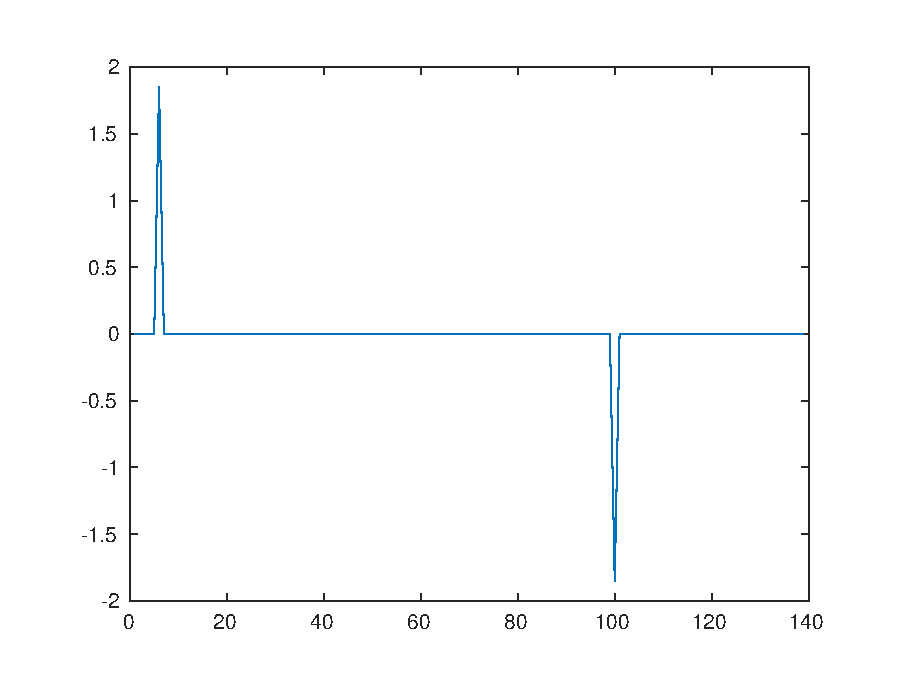
\includegraphics[width=\maxwidth{83.69292523833417em}]{figure_0.eps}
\end{center}

\begin{par}
\begin{flushleft}
 
\end{flushleft}
\end{par}

\begin{par}
\begin{flushleft}
Using the above feedback control to plot the state of the linearized system
\end{flushleft}
\end{par}

\begin{matlabcode}
% define three initial state vector x_0
x_0 = [0; 0; 0; 0];

options_custom = odeset('MaxStep',0.03);
[t,e] = ode45(@(t,e)(lane_controller(e, A, B_1, B_2, K, psi_dot_desired, t)),timespan,x_0, options_custom);

plot(t, e(:,1))
title('e1')
ylabel('Amplitude')
xlabel('time(s)')
\end{matlabcode}
\begin{center}
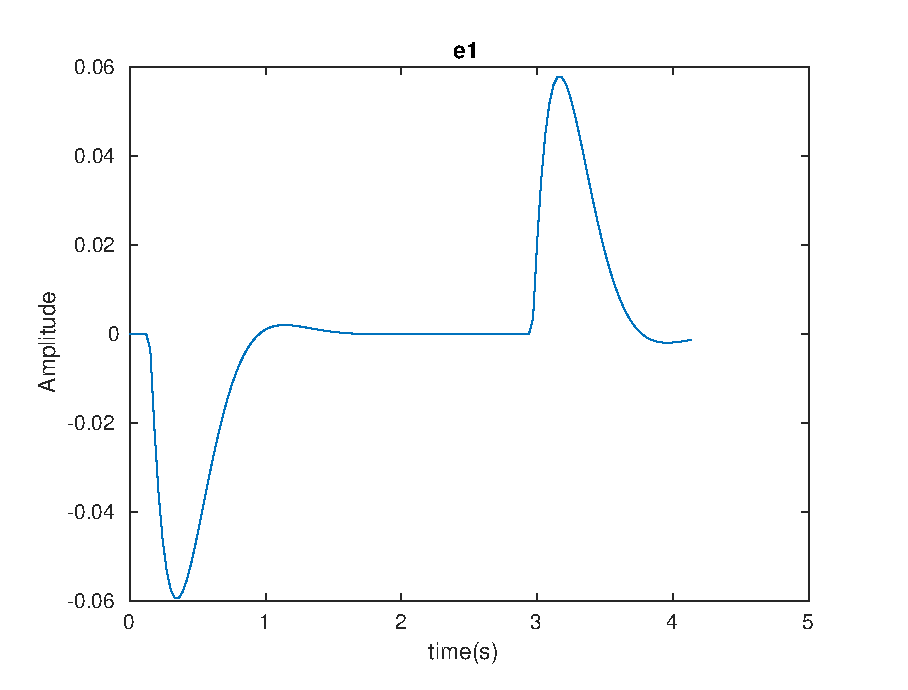
\includegraphics[width=\maxwidth{83.69292523833417em}]{figure_1.eps}
\end{center}
\begin{matlabcode}

% plot(t, e(:,2))
% title('e1 dot')
% ylabel('Amplitude')
% xlabel('time(s)')

plot(t, e(:,3))
title('e2')
ylabel('Amplitude')
xlabel('time(s)')
\end{matlabcode}
\begin{center}
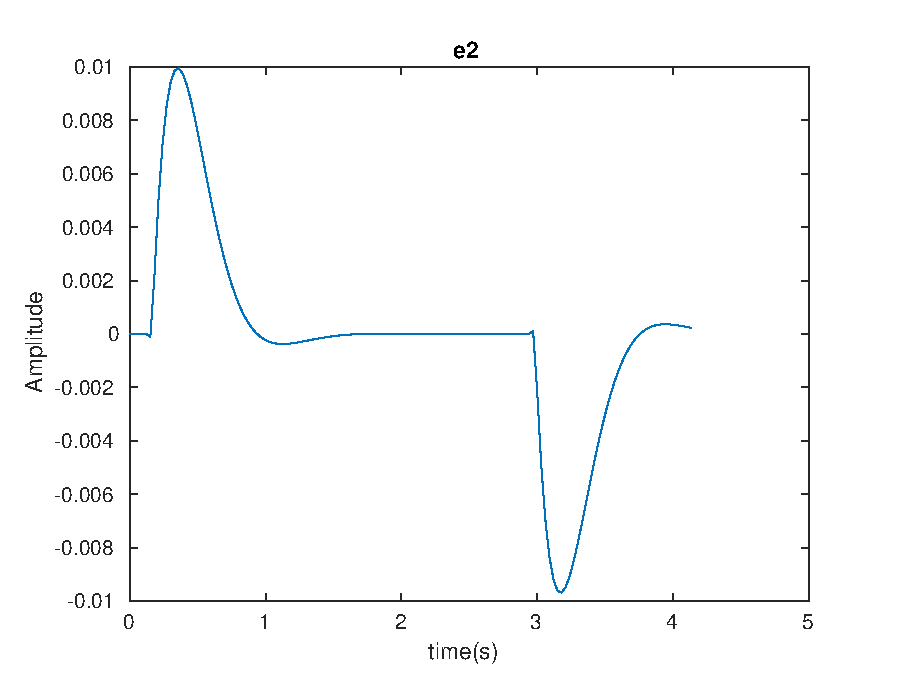
\includegraphics[width=\maxwidth{83.69292523833417em}]{figure_2.eps}
\end{center}
\begin{matlabcode}

% plot(t, e(:,4))
% title('e2 dot')
% ylabel('Amplitude')
% xlabel('time(s)')

[e1_max, index_e1] = max(abs(e(:,1)));
[e2_max, index_e2] = max(abs(e(:,3)));

delta = K*transpose(e);
steer_angle = diff(delta)/0.03;
plot(steer_angle)
title('rate of change of steer angle')
\end{matlabcode}
\begin{center}
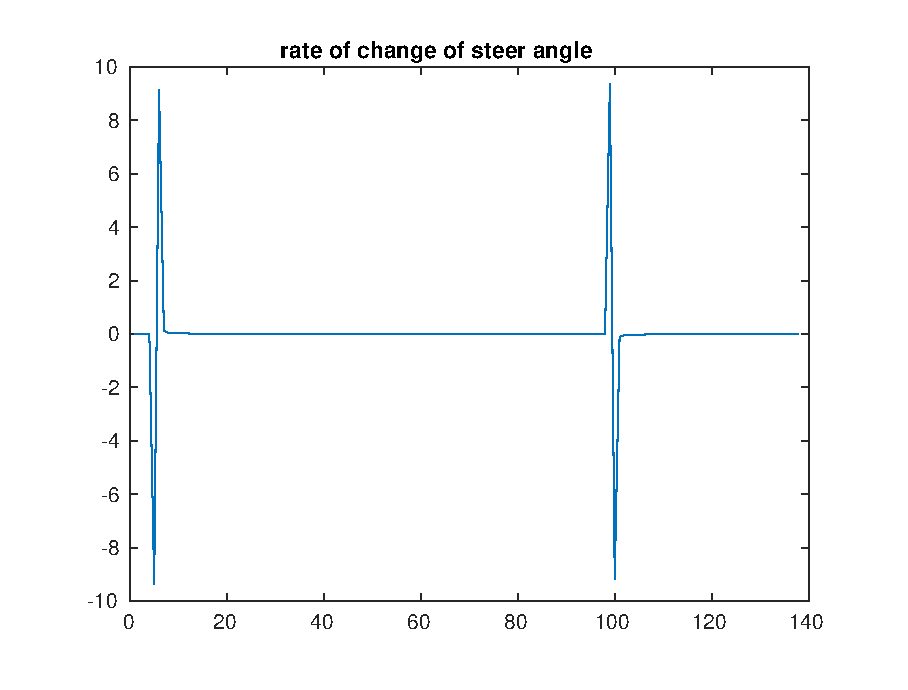
\includegraphics[width=\maxwidth{83.69292523833417em}]{figure_3.eps}
\end{center}
\begin{matlabcode}
% ylabel('Amplitude in rad/s')
% xlabel('time(s)')

maximum_abs_e1_error = e1_max % unit = metres
\end{matlabcode}
\begin{matlaboutput}
maximum_abs_e1_error = 0.0594
\end{matlaboutput}
\begin{matlabcode}
maximum_abs_e2_error = e2_max % unit = radians
\end{matlabcode}
\begin{matlaboutput}
maximum_abs_e2_error = 0.0100
\end{matlaboutput}
\begin{matlabcode}
e1_one_second_after_first_transition = e(int32((t_1+1)/0.03),1)
\end{matlabcode}
\begin{matlaboutput}
e1_one_second_after_first_transition = 0.0020
\end{matlaboutput}
\begin{matlabcode}
e1_one_second_after_second_transition = e(int32((t_1+t_2+1)/0.03),1)
\end{matlabcode}
\begin{matlaboutput}
e1_one_second_after_second_transition = -0.0013
\end{matlaboutput}
\begin{matlabcode}
max_derivative_of_steer_angle = max(abs(steer_angle))
\end{matlabcode}
\begin{matlaboutput}
max_derivative_of_steer_angle = 9.3822
\end{matlaboutput}
\begin{matlabcode}

e2_one_second_after_first_transition = e(int32((t_1+1)/0.03),3)
\end{matlabcode}
\begin{matlaboutput}
e2_one_second_after_first_transition = -3.7357e-04
\end{matlaboutput}
\begin{matlabcode}
e2_one_second_after_second_transition = e(int32((t_1+t_2+1)/0.03),3)
\end{matlabcode}
\begin{matlaboutput}
e2_one_second_after_second_transition = 2.2800e-04
\end{matlaboutput}
\begin{matlabcode}

\end{matlabcode}

\matlabheadingthree{\textbf{-------------------------------------------------------------------------------------------------------------------------------------------------------------------------}}

\matlabheadingthree{2.3 Desired and Actual Plot}

\begin{par}
\begin{flushleft}
\includegraphics[width=\maxwidth{49.8745609633718em}]{image_7}
\end{flushleft}
\end{par}

\begin{matlabcode}
% Define the lateral and longitudinal tracking values in terms of errors
% e = [e1; e1_dot; e2; e2_dot]
e_t = transpose(e);

psi_track = e_t(3,:) + psi_desired;

x_track = x_des - e_t(1,:).*sin(psi_track);
y_track = y_des + e_t(1,:).*cos(psi_track);

% global tracking
plot(x_track, y_track);
title('global tracking')
ylabel('y (metres)')
xlabel('x (metres)')
hold on
plot(x_des, y_des)
legend({'actual tracking', 'desired_track'},'Location','northwest')
hold off
\end{matlabcode}
\begin{center}
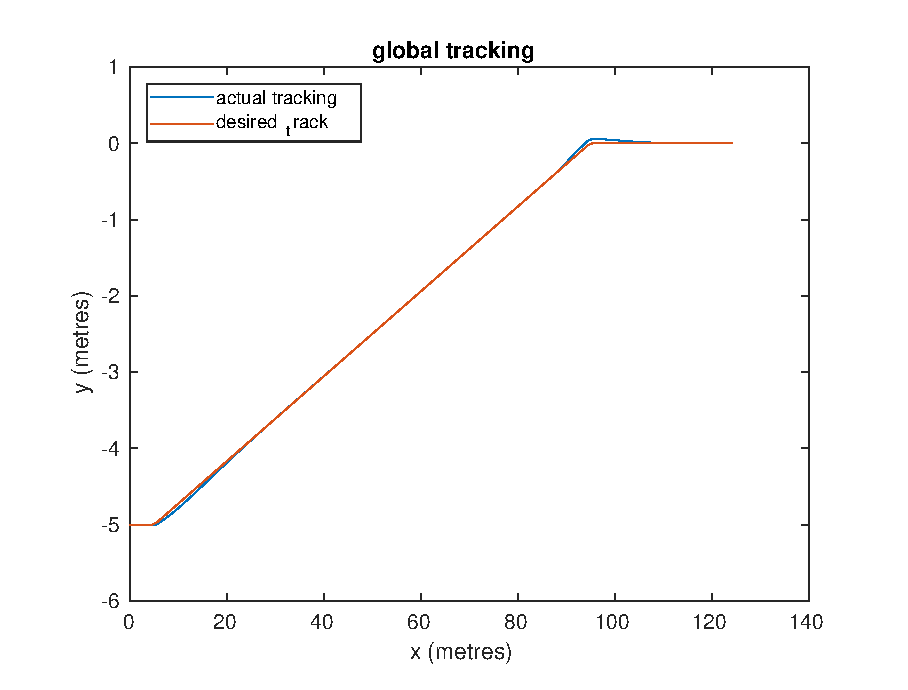
\includegraphics[width=\maxwidth{83.69292523833417em}]{figure_4.eps}
\end{center}

\begin{par}
\begin{flushleft}
---------------------------------------------------------------------------------------------------------------------------------------------
\end{flushleft}
\end{par}

\matlabheadingthree{2.4 Curved Track}

\begin{par}
\hfill \break
\end{par}

\begin{matlabcode}
t_1 = 1;
t_2 = 5;
t_3 = 1;
t_4 = 5;

% Individual timespans
timespan_1 = 0 : 0.03 : t_1;
timespan_2 = (timespan_1(end)+0.03) : 0.03 : t_2+t_1;
timespan_3 = (timespan_2(end)+0.03) : 0.03 : t_1+t_2+t_3;
timespan_4 = (timespan_3(end)+0.03) : 0.03 : t_1+t_2+t_3+t_4;

% Combined timespans with timestep = 0.03
timespan = 0 : 0.03 : (t_1 + t_2 + t_3 + t_4);
\end{matlabcode}


\vspace{1em}
\begin{par}
\begin{flushleft}
Now defining each part of the curve
\end{flushleft}
\end{par}

\begin{matlabcode}
% % define the array which will hold x_des and y_des
% xc_des = [];
% yc_des = [];
% 
% % defining the first straight line path starting at 0,0
% for t1 = timespan_1
%     xc_des(end+1) = 30*t1;
%     yc_des(end+1) = 0;
% end
% 
% % defining the arc with center at 30,1000
% % (x-h)2+(y-k)2 = a2
% % y = (a2 - (x-h)2)^0.5 + k
% for t2 = timespan_2
%     xc_des(end+1) = 30*t2;
%     yc_des(end+1) = sqrt(1000 - (xc_des(end)-30)^2) + 1000;
% end
% 
% % finding the slope of the last timestep in circle to continue the line
% m3 = (yc_des(end)-yc_des(end-1))/(xc_des(end)-xc_des(end-1));
% y_intercep_3 = yc_des(end) - m3*xc_des(end)
% 
% for t3 = timespan_3
%     xc_des(end+1) = 30*t3;
%     yc_des(end+1) = m3*xc_des(end) + y_intercep_3;
% end
% 
% plot(xc_des, yc_des);
\end{matlabcode}


\vspace{1em}
\begin{par}
\begin{flushleft}
Define the psi\_dot\_des, psi\_des, x\_des and y\_des
\end{flushleft}
\end{par}

\begin{matlabcode}
psi_des = [];
psi_dot_des = [];
x_des = [];
y_des = [];

timespan_1(end)
\end{matlabcode}
\begin{matlaboutput}
ans = 0.9900
\end{matlaboutput}
\begin{matlabcode}
timespan_2(end)
\end{matlabcode}
\begin{matlaboutput}
ans = 6
\end{matlaboutput}
\begin{matlabcode}
timespan_3(end)
\end{matlabcode}
\begin{matlaboutput}
ans = 6.9900
\end{matlaboutput}
\begin{matlabcode}
timespan_4(end)
\end{matlabcode}
\begin{matlaboutput}
ans = 12
\end{matlaboutput}
\begin{matlabcode}

% defining psi_dot_des
for t = timespan_1
    psi_dot_des(end+1) = 0;
end

for t = timespan_2
    psi_dot_des(end+1) = V_x/1000; % initial arc with R = 1000 metres
end

for t = timespan_3
    psi_dot_des(end+1) = 0;
end

for t = timespan_4
    psi_dot_des(end+1) = -V_x/500;
end


plot(timespan, psi_dot_des)
title('psi dot des')
\end{matlabcode}
\begin{center}
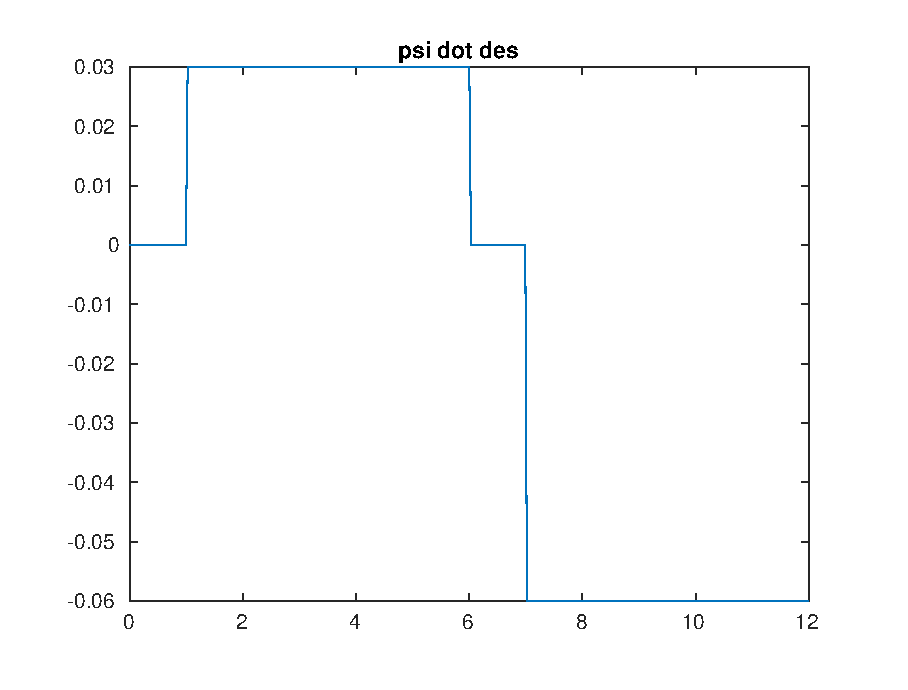
\includegraphics[width=\maxwidth{83.69292523833417em}]{figure_5.eps}
\end{center}
\begin{matlabcode}


% Integrating psi_dot_des to get psi_des
count = 1;
for t=timespan
    if count == 1
        psi_des(count) = 0;
        count = count + 1;
    else
        psi_des(count) = trapz(0.03,psi_dot_des(:,1:count));
        count = count + 1;
    end
end

% integ cos(psi_des) to get x_des
count = 1;
for t=timespan
    if count == 1
        x_des(count) = 0;
        count = count + 1;
    else
        x_des(count) = trapz(0.03,V_x*cos(psi_des(:,1:count)));
        count = count + 1;
    end
end

% integ sin(psi_des) to get y_des
count = 1;
for t=timespan
    if count == 1
        y_des(count) = 0;
        count = count + 1;
    else
        y_des(count) = trapz(0.03, V_x*sin(psi_des(:,1:count)));
        count = count + 1;
    end
end

plot(psi_des);
title('psi des');
\end{matlabcode}
\begin{center}
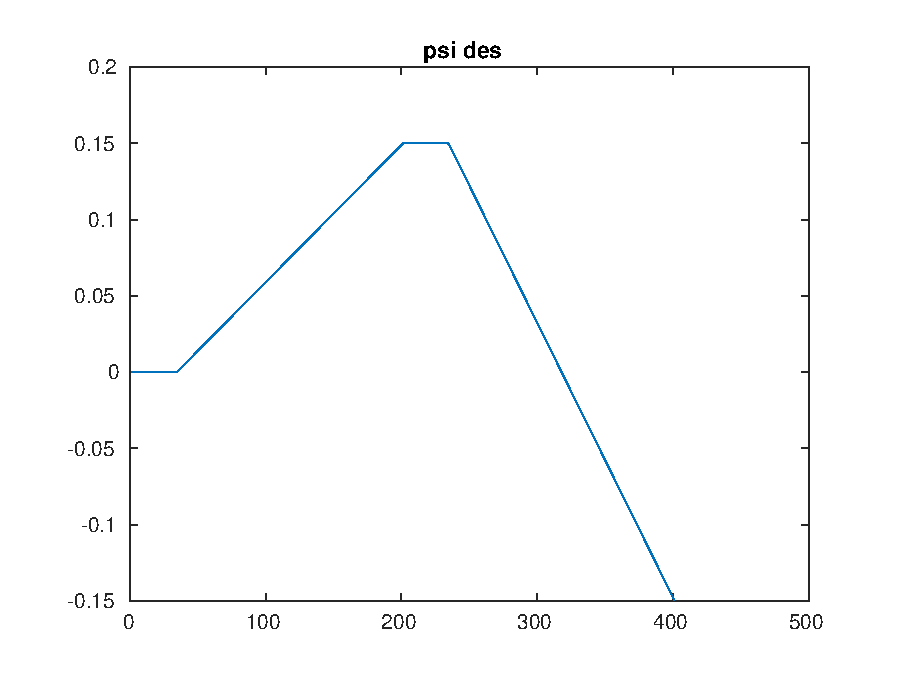
\includegraphics[width=\maxwidth{83.69292523833417em}]{figure_6.eps}
\end{center}
\begin{matlabcode}

plot(x_des, y_des);
title('desired path');
\end{matlabcode}
\begin{center}
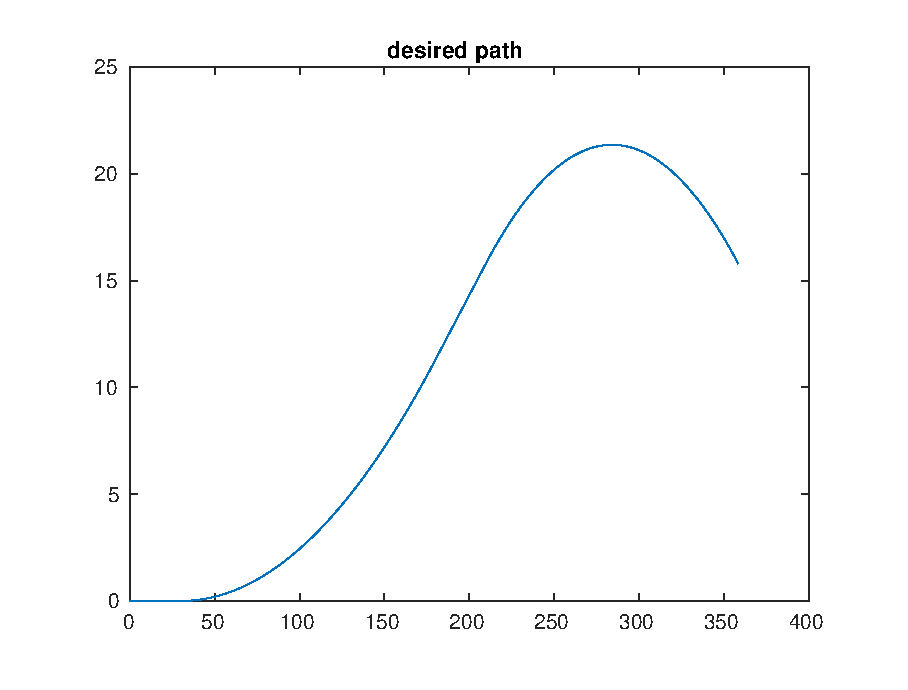
\includegraphics[width=\maxwidth{83.69292523833417em}]{figure_7.eps}
\end{center}


\vspace{1em}
\begin{par}
\begin{flushleft}
Define the state space error
\end{flushleft}
\end{par}

\vspace{1em}

\begin{matlabcode}
Q = [[1,0,0,0];[0,100,0,0];[0,0,1,0];[0,0,0,1]];
R = 1;

K = lqr(A, B_1, Q, R)
\end{matlabcode}
\begin{matlaboutput}
K = 1x4    
    1.0000    9.9156    2.5746    0.0800

\end{matlaboutput}
\begin{matlabcode}

% define three initial state vector x_0
x_0 = [0; 0; 0; 0];

options_custom = odeset('MaxStep',0.03);
[t,e] = ode45(@(t,e)(lane_controller(e, A, B_1, B_2, K, psi_dot_des, t)),timespan,x_0, options_custom);

plot(t, e(:,1))
title('e1')
ylabel('Amplitude')
xlabel('time(s)')
\end{matlabcode}
\begin{center}
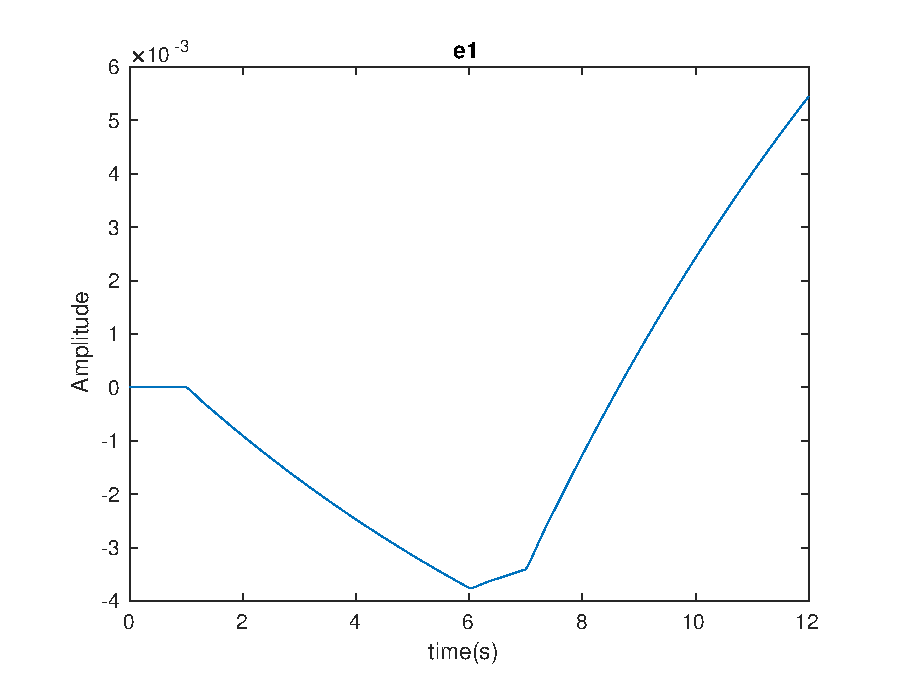
\includegraphics[width=\maxwidth{83.69292523833417em}]{figure_8.eps}
\end{center}
\begin{matlabcode}

% plot(t, e(:,2))
% title('e1 dot')
% ylabel('Amplitude')
% xlabel('time(s)')

plot(t, e(:,3))
title('e2')
ylabel('Amplitude')
xlabel('time(s)')
\end{matlabcode}
\begin{center}
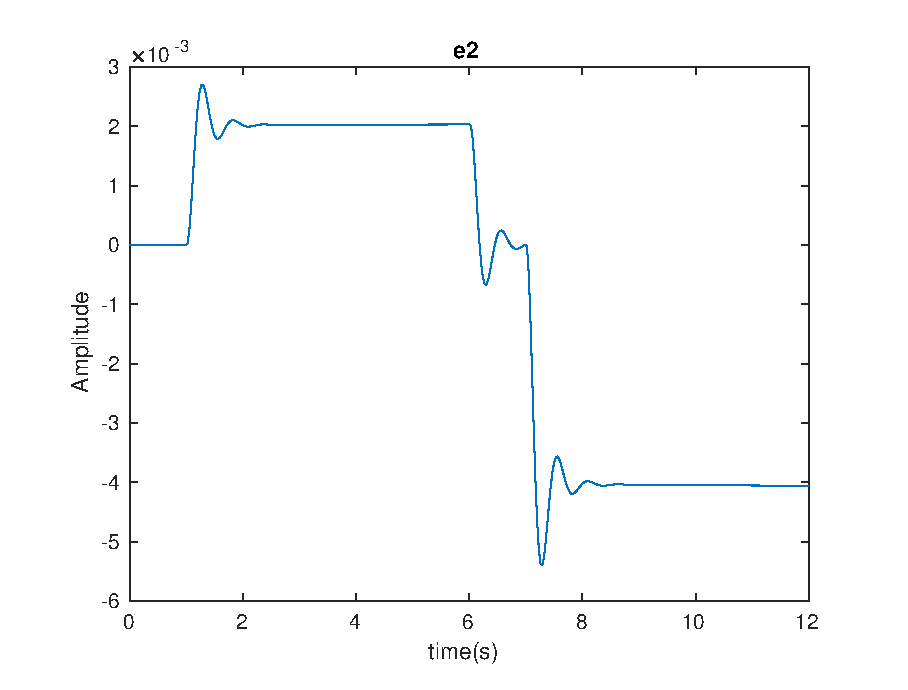
\includegraphics[width=\maxwidth{83.69292523833417em}]{figure_9.eps}
\end{center}
\begin{matlabcode}

% plot(t, e(:,4))
% title('e2 dot')
% ylabel('Amplitude')
% xlabel('time(s)')

[e1_max, index_e1] = max(abs(e(:,1)));
[e2_max, index_e2] = max(abs(e(:,3)));

maximum_abs_e1_error = e1_max % unit = metres
\end{matlabcode}
\begin{matlaboutput}
maximum_abs_e1_error = 0.0054
\end{matlaboutput}
\begin{matlabcode}
maximum_abs_e2_error = e2_max % unit = radians
\end{matlabcode}
\begin{matlaboutput}
maximum_abs_e2_error = 0.0054
\end{matlaboutput}


\vspace{1em}
\begin{par}
\begin{flushleft}
Print the actual and desired plots
\end{flushleft}
\end{par}

\begin{matlabcode}
% Define the lateral and longitudinal tracking values in terms of errors
% e = [e1; e1_dot; e2; e2_dot]
e_t = transpose(e);

x_track = [];
y_track = [];

psi_track = e_t(3,:) + psi_desired;
x_track = x_des - e_t(1,:).*sin(psi_track);
y_track = y_des + e_t(1,:).*cos(psi_track);

% global tracking
plot(x_track, y_track);
title('global tracking')
ylabel('y (metres)')
xlabel('x (metres)')
hold on
plot(x_des, y_des)
legend({'actual tracking', 'desired track'},'Location','northwest')
hold off
\end{matlabcode}
\begin{center}
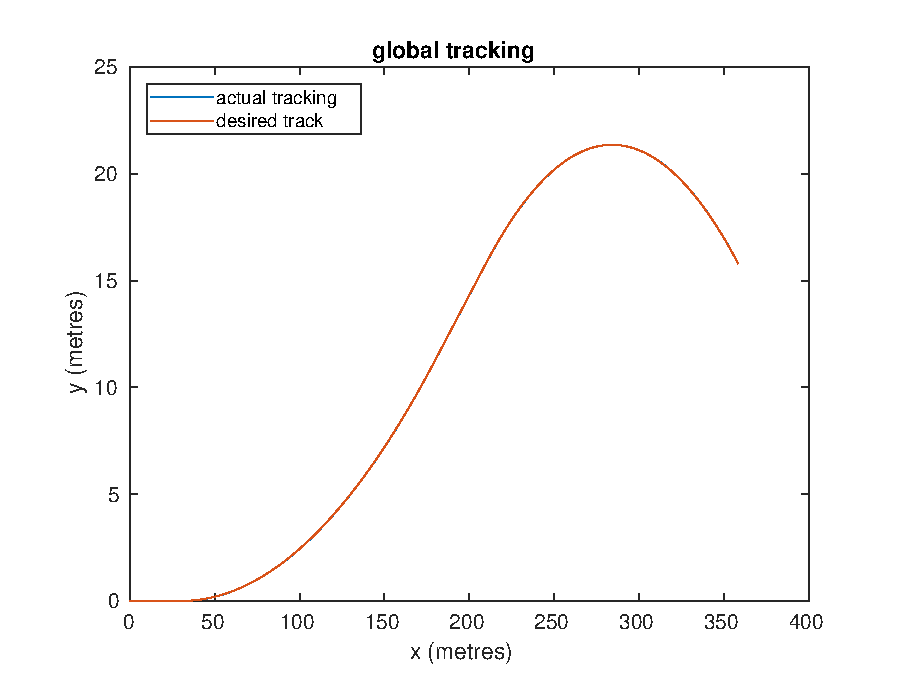
\includegraphics[width=\maxwidth{83.69292523833417em}]{figure_10.eps}
\end{center}



\vspace{1em}
\begin{matlabcode}
function e_dot = lane_controller (e, A, B1, B2, K, psi_dot_des, t)
e1 = e(1);
e1_dot = e(2);
e2 = e(3);
e2_dot = e(4);

i = int32(t/0.03)+1;
psi_dot_des_func = psi_dot_des(i);

e_dot = (A - B1*K)*e + B2*psi_dot_des_func;
end
\end{matlabcode}

\end{document}
